\documentclass[times, 10pt,onecolumn]{article} %
\usepackage{latex8}
\usepackage{times}
\usepackage{url}
\usepackage{amsmath}%
\usepackage{amsfonts}%
\usepackage{amssymb}%
\usepackage{graphicx}
\usepackage{cases}
\usepackage{algorithmic}

%\usepackage{amsfonts, amsthm}

\title{Service-oriented Local and Global Visualization with Sorting On-demand for Climate Data}
\author{
Xusheng Xiao\\
\small{xxiao2@ncsu.edu}\\
\small{Nov 27th, 2010}
}

\begin{document}
\maketitle
\abstract
Huge amount of climate simulation data are collected from different areas (e.g., cities, countries). By understanding and analyzing the data, climate scientists try to predict the trends of the variation of climate both locally and globally. To assist the prediction, exploring visualization of data mining (e.g., histogram) has been used more and more frequently to get a general view ahead of predicting. Additionally, climate experts would like to analyze data by navigating among levels of data ranging from the most summarized (drill-up) to the most detailed (drill-down). To achieve local and global visualization of climate data, there are two major challenges: (1) globally tranferring data is time-consuming and (2) frequently drill-up and drill-down navigation requires computation of same data set multiple times. To address these challenges, we propose a service oriented approach to compute local and global visualization with sorting on-demand for climate data. For global transferring data, our novel approach first asks the data sources to compute local parameters (min, max and count). By collecting these local parameters, our approach computes global parameters and distribute these global parameters to guide local data sources how to compute the histogram data using proper parameters. These computed histogram data from different data sources are then transferred to form a global histogram, whose size is much less than the whole data sets. For data navigation of historgram, our approach caches the transferred data sets and sort only the data in the interval later requested by the data navigation. In this way, we enable climate scientists to navigate huge data sets with acceptable performance. Our preliminary results show that our approach can perform well on sample data sets of climate simulation data.  

\section{Introduction}
\subsection{Motivations} 
Increasing computing power enables modelers to generate larger simulation data sets of climate data from different areas (e.g., cities, countries and continents). Identifying and analyzing patterns in these data sets of climate simulatin data is important, since these patterns help climate scientists develop a deeper understanding of the complex processes contributing to observed phenomena. By understanding and analyzing these data sets of climate data, climate scientists can predict the trends of the variation of climate both locally and globally. 

\begin{figure}[!iht]
\begin{center}
  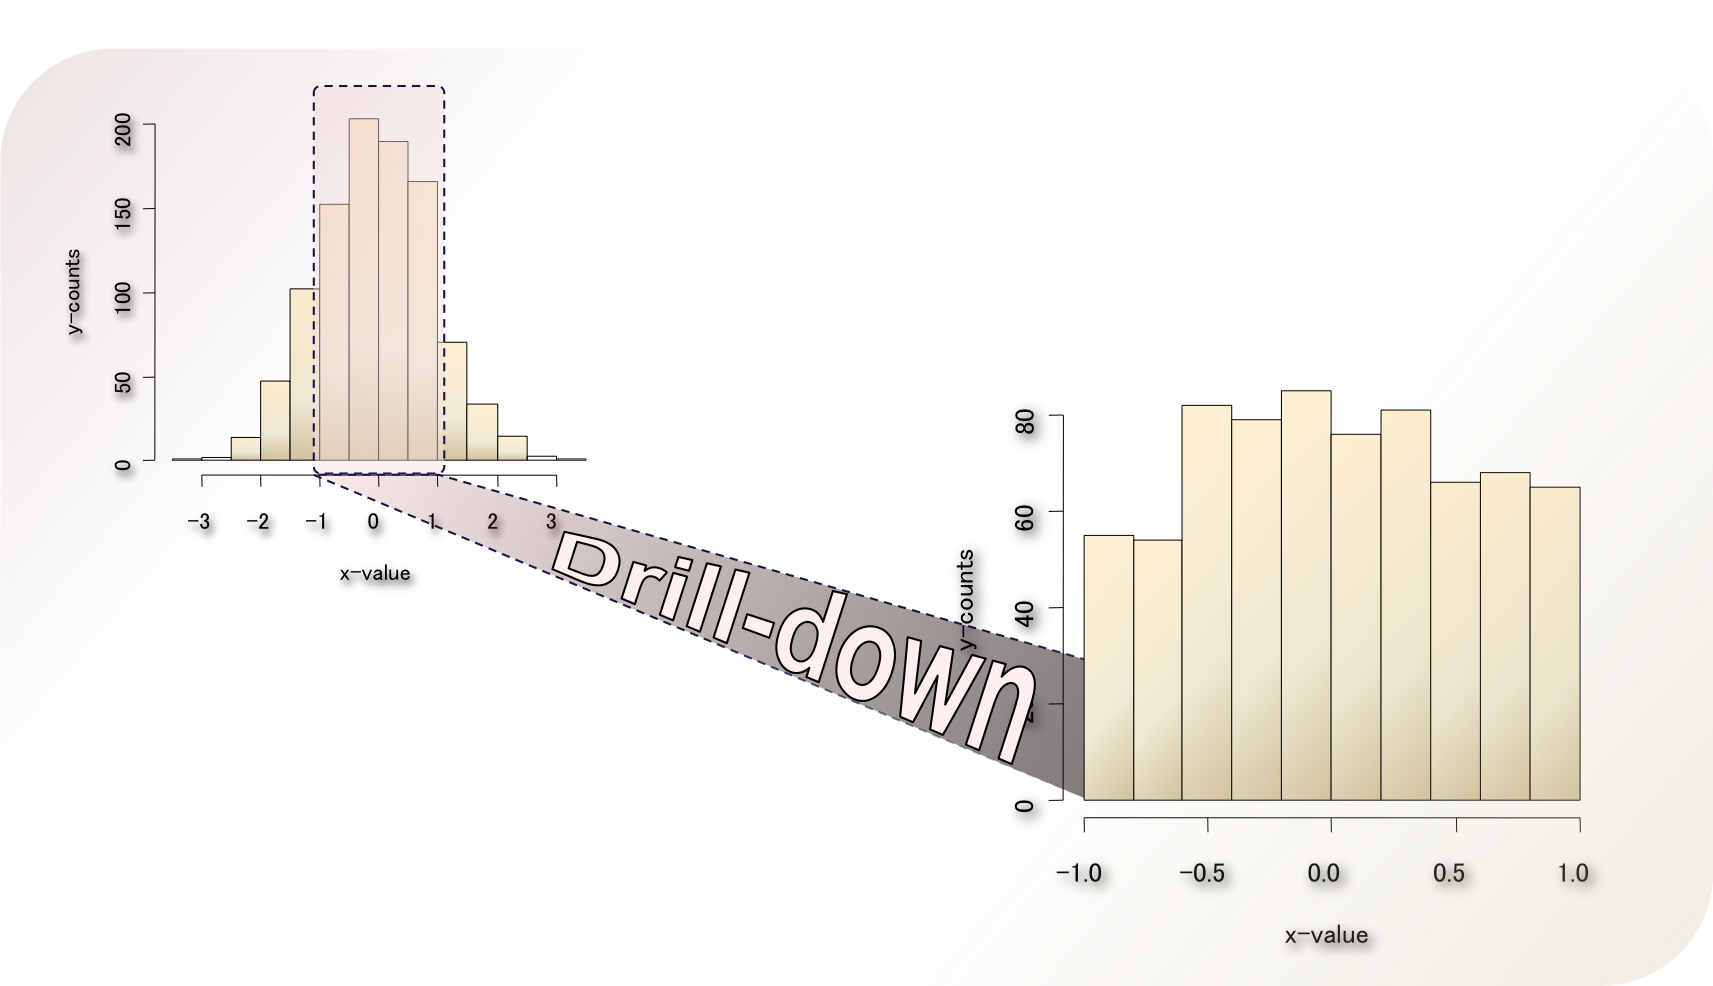
\includegraphics[scale=0.45]{drill.png}
  \caption{Drill-down to interval [-1,1] in histogram}
  \label{fig:drill}
\end{center}
\end{figure}

In order to assist the prediction of the climate variation, exploring visualization of data mining (e.g., histogram~\cite{histogram}) has been used more and more frequently. Showing a global histogram of climate simulation data collected from different data sources can help climate scientists obtain a general view ahead of predicting. However, climate data is well known for its huge amount. In every second, huge amount of climate simulation data is generated from different cities, countries or even thousands of sensors in the same area. The computation for global visualization using histogram normally depends on the distributed computation on different data sources. Hence, there is much need of transferring huge data sets from different data sources with acceptable error rate for computing global visualization. 

%\usepackage{graphics} is needed for \includegraphics

Moreover, to better understand the details of specific areas, climate experts would like to analyze data by navigating among levels of data ranging from the most summarized (drill-up) to the most detailed (drill-down), analogous to navigation in data cube~\cite{datamining}. As we can see in Figure \ref{fig:drill}, the left histogram shows a better global generalization of the distribution of the whole dataset, whereas the right histogram demonstrates a better detailed visualization of the distribution for data with x-value ranges from -1.0 to 1.0. 

\subsection{Challenges} 
In order to visualize climate data sets locally and globally with acceptable performance, there are two major challenges. The first challenge is the high computation time and the unacceptable package loss rate during the global data transferring. Table \ref{tbl:rawdata} shows the synopsis of raw climate data in multiple domains dollected in 2008. As we can see for the data of VOCALS in the table, the data size in 2008 is 3920 MB and transferring this data set requires 10 hours even in best case.

\begin{table}[!iht]
\centering
\begin{tabular}{|c|c|c|c|c|}
\hline
\textbf{Data Domain} & \textbf{Single data set size} & \textbf{\# data sets} & \textbf{Total Size} & \textbf{ Transfer Time In Best Case (Hrs)} \\ \hline
VOCALS 2008 & $\sim$70000 KB & 56 & $\sim$3920 MB & $\sim$10 \\ \hline
HrsASCOS 2008 & $\sim$140000 KB & 25&  $\sim$3500 MB & $\sim$10 \\ \hline 
HrsAEROSE 2008 & $\sim$80000 KB & 36&  $\sim$2880 MB & $\sim$7 \\ \hline 
HrsSTRATUS 2007 & $\sim$70000KB & 21&  $\sim$1470 MB & $\sim$5  \\ \hline
\end{tabular}
\caption{The synopsis of raw climate data in multiple domains collected in 2008.}
\label{tbl:rawdata}
\end{table}

Another challenge is the frequent data navigation of climate data. By drilling-up or drilling-down of the global histogram, we need to recompute the data sets in the specified range, which requires re-transferring the whole data if traditional approach is used. However, Table \ref{tbl:rawdata} already shows that tranferring whole data sets require non-trivial time. Thus, re-transferring whole data set for a navigation is unacceptable. Table \ref{tbl:time} further shows the detailed computation time needed to discovery meaningful or user-specified parameters visualization. As we can see in the table, for the data set of size about 3000 MB, it requires 4 minutes to compute a histogram and 30 times requires 120 minutes, which is far from acceptable performance. 


\begin{table}[!iht]
\centering
\begin{tabular}{|c|c|c|c|}
\hline
\textbf{Data Size} & \textbf{Histogram Execution Time (Once) } & \textbf{Discovery Histogram Execution Time (log(n))} & \textbf{User-specified (30 Times)} \\ \hline
$\sim$1500 MB & 2 Mins & $\sim$17 * 2 = 34 Mins & 60 Mins \\ \hline
$\sim$3000 MB & 4 Mins &  $\sim$18 * 2 = 36 Mins & 120 Mins \\ \hline 
$\sim$4500 MB & 6 Mins &  $\sim$19 * 2 = 38 Mins & 180 Mins \\ \hline 
\end{tabular}
\caption{Total time needed to discovery meaningful or user-specified parameters visualization.}
\label{tbl:time}
\end{table}

\subsection{Solution}
To address these two major challenges, we provide a novel approach, called Service-oriented Local and Global Visualization with Sorting On-demand for Climate Data. Basically, our approach consists of two major steps: 

\begin{itemize}
\item{\textbf{Part I: Service-Oriented Histogram.}} Instead of transferring the whole data sets from different data sources, our approach first locally compute the parameters (min, max and total count of sample data points) based on the requirements of a histogram request. These local data sources then communicates with each other to further compute regional parameters. These regional parameters are processed to compute the global parameters and then re-distribute to each data source for computing the required data sets of local histograms. These local histograms based on the global parameters, whose size is much less than the whole data sets, are finally transferred to compute the global histogram.
\item{\textbf{Part II: On-demand Sorting.}} After transferring the required data sets of local histogram, each data source caches the data sets. When further data navigation requests come in, each data source sorts only the data in the intervals based on the request and recompute a local histogram. These recomputed local histograms are again sent to form a global histogram that fulfills the navigation requirement. 
\end{itemize}


\section{Material and Approach}
\subsection{Data Description}
The Radar Data Information of those projects are stored on a Tb data storage system at PSD in Boulder, CO\footnote{\url{http://www.esrl.noaa.gov/psd/psd3/cruises/}}. The details of data is shown as below.
\begin{itemize}
  \item \textbf{VOCALS 2008:} 915 MHz profiler reflectivity from vertical pointing beam only. These data are from the electronically stabilized system. 
\item \textbf{ASCOS 2008:} 449 MHZ Wind Profiler data; half-hour consensus profile data from the 449 MHz wind profiler on the Oden during ASCOS.  
\item \textbf{AEROSE 2008:} 556 MHZ Wind profiler rbclear AEROSE 2008, one-hour consensus profile data.
\item \textbf{STRATUS 2007:} 778 MHZ Wind profiler rcSNR AMMA 2007, UTC time per hour consensus profile data.
\end{itemize}
\subsection{Data Transmission and Package Loss Ratio}
\textbf{Data transmission, digital transmission or digital communications} is the physical transfer of data (a digital bit stream) over a point-to-point or point-to-multipoint communication channel. Examples of such channels are copper wires, optical fibers, wireless communication channels, and storage media. The data is represented as an electromagnetic signal, such as an electrical voltage, radio-wave, microwave or infrared signal~\cite{PDAT}. 

\textbf{Package Loss} occurs when one or more packets of data travelling across a computer network fail to reach their destination. Packet loss is distinguished as one of the three main error types encountered in digital communications; the other two being bit error and spurious packets caused due to noise\footnote{\url{http://www.nessoft.com/kb/24}}.
\subsection{Histogram}
\subsection{Sort\cite{ps}}
\subsection{New Approach}
\subsubsection{Service-Oriented Framework}
\subsubsection{Sorting Pre-conditioner Histogram}
\section{Result}
\section{Discussion}
\bibliographystyle{unsrt}
\bibliography{references}
\end{document}